\documentclass{standalone}
\usepackage{tikz}
\usetikzlibrary{lindenmayersystems}
\usetikzlibrary[shadings]

\begin{document}
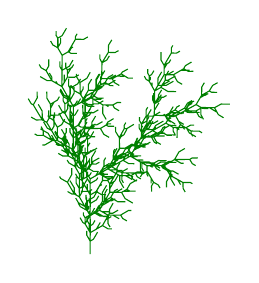
\begin{tikzpicture}
\draw [green!50!black, rotate=90]
[l-system={rule set={F -> FF-[-F+F]+[+F-F]}, axiom=F, order=4, step=2pt,
randomize step percent=25, angle=30, randomize angle percent=5}]
lindenmayer system;
\end{tikzpicture}
\end{document}